% begin module implicit-differentiation-intro
\begin{frame}
\frametitle{Implicit Differentiation}
\begin{itemize}
\item  So far, we have seen functions with formulas that express one varable explicitly in terms of the other.
\item<2->  $y = \sqrt{x^3+1}$, $y = x\sin x$, etc.
\item<3->  Some functions are given implicitly by a relation between $x$ and $y$.
\item<4->  $x^2 + y^2 = 1$ isn't the equation of any one function.
\item<5->  Implicitly it gives two functions: \uncover<6->{$\alert<6>{y = \sqrt{1-x^2}}$ and} \uncover<7->{\alert<7>{$ y = -\sqrt{1-x^2}$}.}
\item<8->  How do we differentiate these functions?
\item<9->  Differentiate both sides with respect to $x$, and then solve for $y'$.
\end{itemize}
\begin{center}
\psset{xunit=1.5cm, yunit=1.5cm}
\begin{pspicture}(-1.8, -1.15)(1.8,1.25)
\tiny
\psaxes[ticks=none, labels=none]{<->}(0,0)(-1.7,-1.15)(1.7,1.2)
\fcLabels{1.7}{1.2}
\uncover<4,5,6,8->{
\psplot[linecolor=\fcColorGraph, plotpoints=1000]{-1}{1}{x 2 exp -1 mul 1 add sqrt }
}
\uncover<7>{
\psplot[linestyle=dashed, linecolor=gray!50, plotpoints=1000]{-1}{1}{x 2 exp -1 mul 1 add sqrt }
}
\uncover<4,5,7,8->{
\psplot[linecolor=\fcColorGraph, plotpoints=1000]{-1}{1}{x 2 exp -1 mul 1 add sqrt -1 mul }
}
\uncover<6>{
\psplot[linestyle=dashed, linecolor=gray!50, plotpoints=1000]{-1}{1}{x 2 exp -1 mul 1 add sqrt -1 mul }
}
\uncover<6->{\rput[l](0.5,1){$y=\sqrt{1- x^{2}}$} }
\uncover<7->{\rput[l](0.5,-1){$y=- \sqrt{1- x^{2}}$} }
\end{pspicture}

%\ \uncover<5->{%
%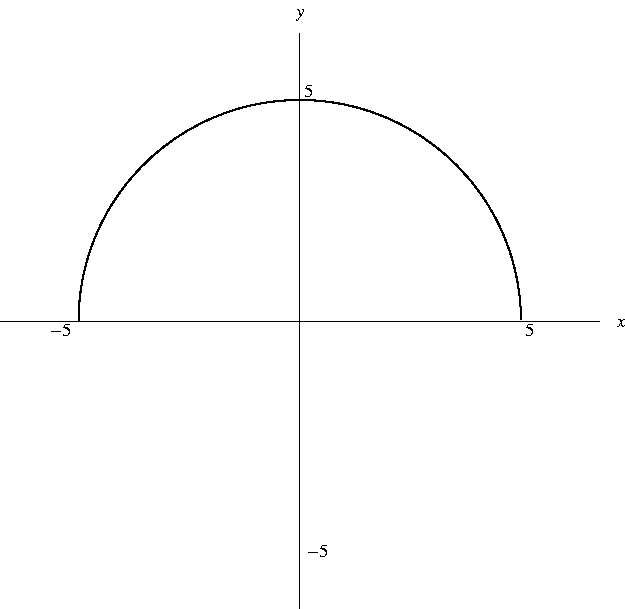
\includegraphics[height=2.5cm]{implicit-differentiation/pictures/03-06-circletop.pdf}%
%}%
%\ \uncover<4->{%
%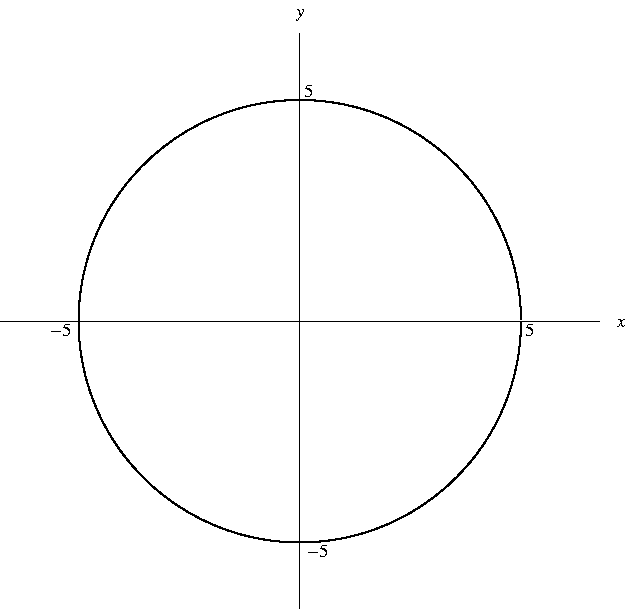
\includegraphics[height=2.5cm]{implicit-differentiation/pictures/03-06-circle.pdf}%
%}%
%\ \uncover<5->{%
%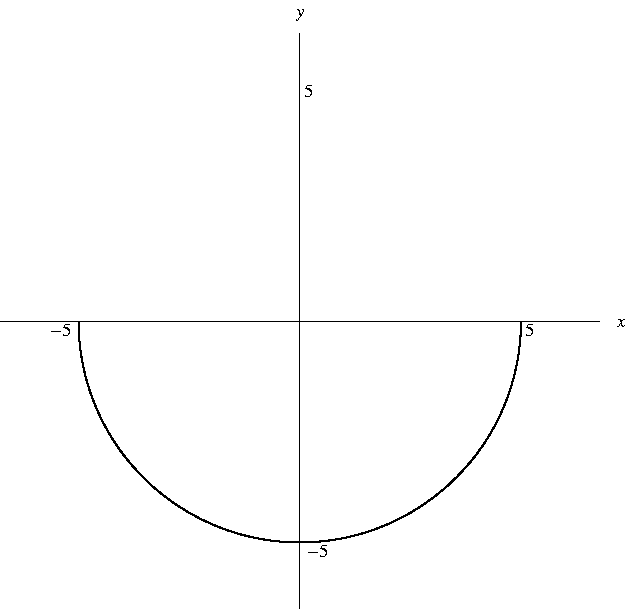
\includegraphics[height=2.5cm]{implicit-differentiation/pictures/03-06-circlebottom.pdf}%
%}%
\end{center}
\end{frame}
% end module implicit-differentiation-intro
